\chapter{Dataset Construction and Experimental Setup}
\label{ch:experimental_setup}
This chapter describes how the datasets used in the experiments were constructed. The process starts from raw Linux conntrack metadata collected from real OT environments. These binary event files are reconstructed into unidirectional flow records, and split chronologically into training, validation, and test periods. Attack data is simulated and remapped to match the companies' data context. The resulting output is therefore a set of flow-level datasets that serve as input to the feature extraction and detection methodology described in Chapter~\ref{ch:detection_methodology}.


% \textcolor{blue}{TOO LONG? SHOULD I DEVIDE THIS INTO TWO CHAPTERS?? split up into set-up/tools and actual pipeline? Or just split it into two as it is so it doesn't feel like I am repeating myself?}

\section{Data Source and Scope}



\subsection{Linux Connection Tracking Metadata}

This thesis was carried out in collaboration with AXS Guard, a Belgian cybersecurity company based in Mechelen~\cite{axs_guard_meet_nodate}. AXS Guard develops and manages cybersecurity solutions for organizations of all types, with a focus on security gateways and managed cybersecurity services. They provided the real network metadata used in this thesis, which originates from operational customer environments and therefore represents realistic OT communication patterns.

The metadata was collected from AXS Guard appliances deployed at the network edge, where they operate as routers and firewalls. This deployment context is important for the design of the dataset. The appliances must perform their primary networking and security functions continuously, while operating under hardware constraints that depend on the specific model. Some appliances have limited memory resources, starting from 1 GB on the least performant models, and going up to 12 GB or 16 GB of memory~\cite{axs_guard_product_2026}. These constraints motivate the use of lightweight network metadata rather than packet payloads or host-level process information.

For this reason, the dataset is based on Linux conntrack metadata. Conntrack is the connection-tracking subsystem of the Linux kernel and is part of the Netfilter framework. It maintains metadata about observed network flows, such as source and destination addresses, ports, protocol, packet and byte counters, timestamps, and connection state. Conntrack is commonly used by firewalling and NAT systems such as iptables and nftables, but in this thesis it is used only as a source of lightweight network-flow metadata for anomaly detection~\cite{neira2006conntrack,netfilter_nftables_2025}. Since conntrack is already natively integrated into the Linux networking stack, it allows the system to passively extract useful network visibility without requiring complex network reconfiguration or additional heavyweight monitoring components.

The dataset should therefore be interpreted as network connection metadata observed at the monitored subnet or gateway. It does not provide a complete view of all communication in the customer organization, but only of the traffic visible from the selected observation point. It also does not contain packet payloads, sensor readings, actuator states, PLC register values, or other process-level variables. Instead, the analysis in this thesis is based on metadata describing communication patterns between endpoints.



\subsection{Data Confidentiality \& Limitations}
\label{sec:data_lim_conf}

The datasets used come from real OT environments of the collaborating companies. Because these environments are operationally sensitive, several details are intentionally omitted or anonymized. This includes the names of the companies, exact network topologies, device roles, raw IP addresses, and any information that could reveal the structure or operation of the industrial networks. Where examples are shown, synthetic or anonymized values are used.


For safety and operational reasons, reconnaissance attacks were not executed directly against the OT environments. Even what looks like harmless scanning activity can disrupt fragile or legacy industrial devices, trigger alerts, or interfere with normal operations. Instead, reconnaissance behavior was simulated in a controlled environment and injected into the real benign traffic. This approach allows the evaluation of attack detection methods while avoiding unnecessary risk to customer systems.
% \textcolor{red}{add dummy data example}
\subsection{Data Scope}
The OT dataset consists of metadata collected from two real environments. The collected traffic represents normal operational communication observed during the measurement periods.\textcolor{red}{ No confirmed "attacks" were present in the collected company data,} therefore the original OT traffic is treated as benign. The data was collected during the months of March and April.
\textcolor{red}{talk about anomalies in training data }

\section{Data Pre-processing}
\textcolor{blue}{is this too much information?? Too many tables?}

\subsection{Conntrack Ingestion}

\textcolor{blue}{credit Enrique for this? how?}

The raw conntrack data was logged as compressed binary event files. Each file contains a sequence of conntrack events rather than already finalized flow records. Therefore, the first preprocessing step was to decompress the files and parse the binary event stream into structured records.

\begin{table}[htbp]
\centering
\scriptsize
\caption{Preview of raw conntrack events (anonymized).}
\label{tab:raw_conntrack_preview}
\makebox[\textwidth][c]{%
\begin{tabular}{llllllll}
\toprule
Event & Conn. ID & Timestamp & L4 & Source IP & Destination IP & Orig. Bytes & Reply Bytes \\
\midrule


LIST & 105672107 & 2026-03-19 13:54:39.559 & 6 & 10.20.109.217 & 10.20.37.127 & 422 & 1421 \\
LIST & 3843433871 & 2026-03-19 13:54:39.559 & 6 & 10.20.109.217 & 10.20.235.187 & 422 & 1551 \\
DELETE & 4122098797 & 2026-03-19 13:54:39.582 &  & nan & nan & 422 & 1048 \\
ADD & 4122098797 & 2026-03-19 13:54:39.582 & 6 & 10.20.109.217 & 10.20.146.19 & 0 & 0 \\
ADD & 1297319782 & 2026-03-19 13:54:39.638 & 6 & 10.20.109.217 & 10.20.10.241 & 0 & 0 \\
DELETE & 923955930 & 2026-03-19 13:54:40.343 &  & nan & nan & 422 & 1666 \\
DROP & 28924 & 2026-03-19 13:54:56.343 & 17 & 10.20.85.60 & 10.20.144.114 & 64 &  \\
DROP & 0 & 2026-03-19 13:54:56.343 & 6 & 10.20.3.179 & 10.20.199.224 & 40 &  \\
UPDATE & 711927862 & 2026-03-19 14:04:39.553 &  & nan & nan & 462 & 1492 \\

\bottomrule
\end{tabular}
}
\end{table}


Table~\ref{tab:raw_conntrack_preview} shows a small preview of the raw event stream after decompression and initial parsing. The parser processes the event stream sequentially and maintains a dictionary of active connections indexed by connection identifier. \texttt{ADD} events initialize new active
connections using the available packet metadata. \texttt{UPDATE}  events provide intermediate cumulative byte and packet counters
for an active connection, while \texttt{DELETE} events finalize connections using the end timestamp and final byte and packet counters. \texttt{LIST}, \texttt{EMPTY}, \texttt{HEADER}, and \texttt{DROP} events are skipped because they do not describe a connection state transition that can be mapped to a reconstructed flow record.  \texttt{HEADER} events contain stream-level metadata, \texttt{EMPTY} events contain no connection data, \texttt{LIST} events are used for listing existing conntrack entries, and \texttt{DROP} events indicate records that were discarded.

The resulting finalized connections, initially produced in connection-completion order, are converted into unidirectional flow records and sorted chronologically by start time in order to preserve information about communication directionality. Important characteristics of reconnaissance are not just the existence of a connection, but also by which host initiated the communication, which hosts or ports were targeted, and whether the probing activity received responses. Table~\ref{tab:sorted_unidirectional} provides an example of flow produced by this preprocessing step.

\begin{table}[htbp]
\centering
\scriptsize
\caption{Preview of reconstructed unidirectional conntrack flows (anonymized).}
\label{tab:sorted_unidirectional}
\makebox[\textwidth][c]{%
\begin{tabular}{llllllllll}
\toprule
\makecell{Start\\Time} &
\makecell{End\\Time} &
L4 &
Src. IP &
Src. Port &
Dst. IP &
Dst. Port &
Bytes &
Packets &
Orig. Direction \\
\midrule
\makecell[l]{2026-03-19\\13:54:39.582} &
\makecell[l]{2026-03-19\\13:56:43.254} &
6 & 10.10.109.217 & 47282 & 10.10.144.114 & 80 & 462 & 7 & True \\

\makecell[l]{2026-03-19\\13:54:39.582} &
\makecell[l]{2026-03-19\\13:56:43.254} &
6 & 10.10.144.114 & 80 & 10.10.109.217 & 47282 & 1940 & 7 & False \\

\makecell[l]{2026-03-19\\13:54:39.638} &
\makecell[l]{2026-03-19\\13:56:43.251} &
6 & 10.10.109.217 & 56620 & 10.10.10.241 & 80 & 422 & 6 & True \\

\makecell[l]{2026-03-19\\13:54:39.638} &
\makecell[l]{2026-03-19\\13:56:43.251} &
6 & 10.10.10.241 & 80 & 10.10.109.217 & 56620 & 1615 & 6 & False \\

\makecell[l]{2026-03-19\\13:54:39.664} &
\makecell[l]{2026-03-19\\13:56:43.224} &
6 & 10.10.146.19 & 80 & 10.10.109.217 & 49516 & 1908 & 7 & False \\

\makecell[l]{2026-03-19\\13:54:39.664} &
\makecell[l]{2026-03-19\\13:56:43.224} &
6 & 10.10.109.217 & 49516 & 10.10.146.19 & 80 & 423 & 6 & True \\

% \makecell[l]{2026-03-19\\13:54:39.680} &
% \makecell[l]{2026-03-19\\13:56:43.240} &
% 6 & 10.10.109.217 & 45888 & 10.10.37.127 & 80 & 422 & 6 & True \\

% \makecell[l]{2026-03-19\\13:54:39.680} &
% \makecell[l]{2026-03-19\\13:56:43.240} &
% 6 & 10.10.37.127 & 80 & 10.10.109.217 & 45888 & 1773 & 6 & False \\

% \makecell[l]{2026-03-19\\13:54:39.824} &
% \makecell[l]{2026-03-19\\13:56:43.258} &
% 6 & 10.10.199.224 & 80 & 10.10.109.217 & 58906 & 880 & 5 & False \\

% \makecell[l]{2026-03-19\\13:54:39.824} &
% \makecell[l]{2026-03-19\\13:56:43.258} &
% 6 & 10.10.109.217 & 58906 & 10.10.199.224 & 80 & 414 & 6 & True \\
\bottomrule
\end{tabular}
}
\end{table}

\subsection{Data Splitting}
After ingestion, the benign company traffic was divided into training, validation, and test periods using a 70--15--15 chronological split. The split was performed at the conntrack-flow level before feature extraction. This was done because of the usage of multiple window sizes during model comparison. If the data were first converted into window-level features and only then split, the exact train, validation, and test periods could depend on the chosen window length. Splitting the underlying flow records first, ensures that all feature extraction runs are based on the same temporal data partitions, making results across different window sizes comparable.

The split was also performed before attack injection, as described in Section~\ref{sec:attack_injection}. This ensures that the training set remains free of simulated attack traffic, which is important for the semi-supervised approach of the thesis, ensuring the models will be trained on data representing purely normal behavior of the targeted environment. The validation and test splits are used as benign background traffic with only them having malicious traces injected. The validation data is used for model selection, threshold tuning, and feature/window configuration choices, while the test data is kept separate for the final performance evaluation.





\section{Attack Simulation}
\label{sec:attack_injection}
\subsection{Attack Environment}


\begin{figure}[htbp]
    
    \centering
    % This automatically scales the diagram to fit the width of your text block
    \resizebox{\textwidth}{!}{%
        \label{fig:env_diagram}
        \begin{tikzpicture}[
    node distance=1.5cm and 1.2cm, 
    % --- BASE STYLES ---
    box/.style={rectangle, rounded corners, inner sep=5pt, align=center, font=\small, minimum height=0.9cm, text width=2.8cm, thick},
    hub/.style={circle, minimum size=2.8cm, align=center, font=\small\bfseries, thick},
    line/.style={draw=black!60, thick}, 
    iplabel/.style={font=\scriptsize, inner sep=2pt, text=black!80}, 
    node sub/.style={label={[font=\small, text=black!80]below:{#1}}},    
    % --- UNIFIED ZONE-BASED COLOR PALETTE ---
    % UNIFIED IT (AMBER ZONE)
    ithubnet/.style={hub, fill=orange!15, draw=orange!60!black},
    itnode/.style={box, fill=orange!10, draw=orange!50!black},    
    % BOUNDARY / DMZ (BLUE)
    boundarynet/.style={box, fill=blue!12, draw=blue!60!black, text width=2.4cm},    
    % NEUTRAL MONITOR (GRAY)
    monitornode/.style={box, fill=gray!15, draw=gray!50!black, text width=2.6cm},    
    % UNIFIED OT (PURPLE ZONE)
    othubnet/.style={hub, fill=purple!15, draw=purple!60!black},
    otnode/.style={box, fill=purple!10, draw=purple!50!black}
]

% ==========================================
% LEFT SIDE (UNIFIED AMBER IT ZONE)
% ==========================================
\node[itnode, node sub={:6081}] (hmi) {HMI\\(Scada LTS)};
\node[itnode, node sub={:6088}, below=1.8cm of hmi] (attacker) {Attacker\\(Kali)};
\node[ithubnet, right=1.6cm of attacker, yshift=0.9cm] (it_hub) {IT\\192.168.90.0/24};

% Clean right-angle bus for HMI and Attacker
\coordinate (it_in) at ($(it_hub.west) + (-0.5cm, 0)$);
\draw[line] (hmi.east) -- node[iplabel, above] {.107} (hmi.east -| it_in) -- (it_in);
\draw[line] (attacker.east) -- node[iplabel, above] {.6} (attacker.east -| it_in) -- (it_in);
\draw[line] (it_in) -- (it_hub.west);

% ==========================================
% MIDDLE (BLUE BOUNDARY & GRAY MONITOR)
% ==========================================
\node[boundarynet, node sub={:5000}, right=1.2cm of it_hub] (router) {Router};

% --- Conntrack Viewer (GRAY, RETURNED to original position) ---
% Positioned directly below the Router, showing its function as a central monitor.
\node[monitornode, node sub={:8001}, below=1.5cm of router] (conntrack) {Conntrack Viewer};

% Connections to Boundary elements
\draw[line] (it_hub.east) -- node[iplabel, pos=0.5, anchor=south] {.200} (router.west);
% Tapping point for the monitor at the boundary
% \draw[line] ($(router.west) + (0.5cm, 0)$) |- (conntrack.west);

% ==========================================
% RIGHT SIDE (UNIFIED PURPLE OT ZONE)
% ==========================================
\node[othubnet, right=1.2cm of router] (ot_hub) {OT\\192.168.95.0/24};
\draw[line] (router.east) -- node[iplabel, pos=0.5, anchor=south] {.200} (ot_hub.west);

% ==========================================
% OT DEVICES
% ==========================================
\node[otnode, node sub={:8080}, right=1.5cm of ot_hub] (plc) {PLC};
\node[otnode, node sub={:6080}, below=1cm of plc] (workstation) {Workstation};

\draw[line] (ot_hub.east) -- node[iplabel, pos=0.6, anchor=south] {.2} (plc.west);
\draw[line] (ot_hub.340) -- ++(0.6cm, 0) |- node[iplabel, pos=0.8, anchor=south] {.5} (workstation.west);

% ==========================================
% SIMULATION GROUP
% ==========================================
\node[draw=violet!80!black, 
      fill=white, 
      dashed, 
      rounded corners, 
      minimum width=6cm, 
      minimum height=9.4cm, 
      above=1cm of plc, 
      anchor=south, 
      very thick] (sim_group) {};

\node[font=\small\bfseries, text=violet!80!black, anchor=south, yshift=0.1cm] at (sim_group.north) {Simulation};
\node[iplabel, anchor=north] at ($(sim_group.south) + (1cm, -0.1cm)$) {:80};

% Bus Line 
\coordinate (sim_bus_top) at ($(sim_group.north west) + (0.8cm, -0.5cm)$);
\coordinate (sim_bus_bottom) at ($(sim_group.south west) + (0.8cm, 0.4cm)$); 
\draw[line] (sim_bus_top) -- (sim_bus_bottom);

% Simulation Nodes: Styles are set implicitly via otnode (purple zone)
\node[otnode, anchor=west] (feed1) at ($(sim_bus_top) + (1.5cm, -0.8cm)$) {Feed 1};
\node[otnode, anchor=west, below=0.5cm of feed1] (feed2) {Feed 2};
\node[otnode, anchor=west, below=0.5cm of feed2] (purge) {Purge};
\node[otnode, anchor=west, below=0.5cm of purge] (product) {Product};
\node[otnode, anchor=west, below=0.5cm of product] (tank) {Tank};
\node[otnode, anchor=west, below=0.5cm of tank] (analyzer) {Analyzer};

% Connect to bus
\foreach \n/\label in {feed1/.10, feed2/.11, purge/.12, product/.13, tank/.14, analyzer/.15} {
    \draw[line] (\n.west) -- node[iplabel, pos=0.7, anchor=south] {\label} (\n.west -| sim_bus_top);
}

% Connect OT Hub UP to the bus
\draw[line] (ot_hub.north) |- (sim_bus_bottom);

\end{tikzpicture}%
    }
    \caption{GRFICSv3 Network Diagram}
\end{figure}
Due to the safety and operational concerns discussed in~\ref{sec:data_lim_conf}, the reconnaissance attacks were not executed against the companies' OT environments. Instead, they were simulated in a virtual OT lab based on the open-source GRFICSv3 environment~\cite{grficsv3_2026}. GRFICSv3 is a containerized ICS/OT cyber-physical security lab that simulates an industrial chemical plant.

The attacks were run from the Kali attacker container (\texttt{192.168.90.6}) which, as shown in Figure~\ref{fig:env_diagram}, is located in the IT network. This represents the scenario where an attacker has obtained control over an IT-side host and performs reconnaissance towards the OT environment. The router/firewall container acts as the observation point, collecting all conntrack metadata form the crossing traffic

\textcolor{red}{the first stage of the Cyber Kill Chain (CKC)\cite{Yadav_2015}}. 

\subsection{Attack Scenarios}
The simulated attacks were designed to represent different forms of reconnaissance. The goal was to generate traffic patterns associated with host discovery, port discovery, service probing, and low-rate scanning. 

The scenarios vary in scan intensity and target scope. Some scans target the full OT subnet, while others target a smaller set of known live OT hosts. The full OT subnet corresponds to \texttt{192.168.95.0/24}. The selected live-host target set consists of known active hosts in the virtual OT network, including \texttt{192.168.95.2}, \texttt{192.168.95.5}, and
\texttt{192.168.95.10--192.168.95.15}. The simulated attacks are summarized in Table~\ref{tab:attack_scenarios}.

\begin{table}[h]
    
    \centering
    \caption{Overview of simulated reconnaissance attack types.}
    \label{tab:attack_scenarios}
    \makebox[\textwidth][c]{
    \begin{tabular}{lll}
        \hline
        Attack type & Scan configuration & Target scope \\
        \hline
        Aggressive subnet scan
            & \texttt{nmap -sS -Pn -T5 --top-ports 100}
            & Full OT subnet \\

        Fast subnet scan
            & \texttt{nmap -sS -Pn -T4 --top-ports 100/200}
            & Full OT subnet \\

        Default-speed subnet scan
            & \texttt{nmap -sS -Pn -T3 --top-ports 100}
            & Full OT subnet \\

        Slow subnet scan
            & \texttt{nmap -sS -Pn -T2 --top-ports 50/100}
            & Full OT subnet \\

        Very Slow targeted scan
            & \texttt{nmap -sS -Pn -T1 -p selected ports}
            & Selected live OT hosts \\

        Extremely slow targeted scan
            & \texttt{nmap -sS -Pn -T0 -p selected ports}
            & Selected live OT hosts \\

        Service/version detection
            & \texttt{nmap -sV -Pn -p selected ports}
            & Selected live OT hosts \\

        Host discovery
            & \texttt{nmap -sn}
            & Full OT subnet \\

        Low-and-slow scan
            & \texttt{nmap -sS -Pn -T2 --top-ports 50}
            & Full OT subnet \\
        \hline
    \end{tabular}
    }
\end{table}

For scanning nmap was selected because it is a widely used network scanning tool for host discovery, port scanning, and service identification, making it suitable for generating controlled reconnaissance traffic with configurable scan intensity and timing~\cite{nmap_nmap_nodate}. Most port discovery scenarios use TCP SYN scanning (\texttt{-sS}) with host discovery disabled (\texttt{-Pn}), so Nmap proceeds directly to probing the specified targets. The timing templates range from very aggressive (\texttt{-T5}) to extremely slow (\texttt{-T0}), allowing the dataset to include both faster and slower reconnaissance behavior. The low-and-slow scenario is included as an Advanced Persistent Threat (APT) inspired reconnaissance pattern, where probing activity is spread over a longer and interrupted period rather than concentrated in a short scan burst.

The selected port sets include common administrative and web ports such as
\texttt{22}, \texttt{80}, and \texttt{443}. They also include OT-relevant
services, most notably Modbus/TCP on port \texttt{502}. Modbus/TCP is commonly
used for supervision and control of automation equipment over TCP/IP networks,
and port \texttt{502} is frequently treated as the default Modbus/TCP port in
ICS scanning and measurement studies~\cite{ortega-fernandez_network_2024, cabana_detecting_2019}. In some runs, port \texttt{8080} was also included to cover web-based industrial interfaces.

Additional scenarios include host discovery (\texttt {-sn}), which identifies reachable devices in the target network without performing a full port scan. Service/version detection (\texttt{-sV}) is also performed as a later reconnaissance step where the scanner attempts to identify the applications or protocols running behind exposed ports\textcolor{red}~\cite{nmap_nmap_nodate}. 


\subsection{Attack Injection}
After executing the described reconnaissance attack scenarios, the adversarial traffic had to be isolated from the benign simulation traffic. This isolation was
based on the recorded attack timelines, the known attacker address, and the target scope of each scenario. Conntrack records were flagged as malign when their timestamps fell within the corresponding attack interval and their endpoints matched the expected bidirectional attacker-to-target communication. 

The isolated attack traces could not be directly inserted into the company data, since much of their metadata would not match. Specifically, the IP addresses and the timestamps from the virtual OT lab had to be modified in order to blend in. The IP remapping was deterministic, ensuring that attacker-side and target-side addresses were projected consistently onto IT-side and OT-side
company ranges, respectively. This preserves the intended attack direction of an IT host performing reconnaissance towards OT targets. The timestamps of the isolated attack traces were also shifted into the relevant periods of the company data. The relative timing within each attack was preserved, so that scan bursts, idle gaps, and low-and-slow patterns remained intact after injection.

After data remapping, the malicious data could be successfully injected into the validation and testing splits. Labels were assigned during this integration step. Original company traffic was treated as benign, while the injected reconnaissance records were labeled as malign traffic. The different attack names were also retained as metadata allowing us to later evaluate our results at a per attack scenario. 

It should be noted that while this is a good approximation of how reconnaissance attacks will look in the different customer environments, it does not fully reproduce all effects of an attack executed directly inside the companies' networks, such as device-specific responses, firewall behavior, or operational side effects.

\chapter{Detection Methodology}
\label{ch:detection_methodology}

% \section{Feature Engineering}
\section{Windowing}
The split, sorted and unidirectional labeled conntrack flows cannot be used directly for model training. Instead, they were aggregated into features representing flow properties over a fixed-length time windows in order to describe the communication behavior of each source host over time. 


Each model input is defined by a source IP address, a timestamp and a window length. In other words, all flows related to the same source host within that same time window are aggregated into one feature vector. For example, when using a 60-minute window, all flows associated with some source host \texttt{10.20.109.217} from 10:00 to 11:00 are combined into one vector containing features such as the number of contacted destination IPs, destination ports, protocol distribution, and packet or byte statistics. An example can be seen in Table~\ref{tab:feature_vector_preview}.

\begin{table}[htbp]
\centering
\caption{Example feature vectors after window-based aggregation.}
\label{tab:feature_vector_preview}
\small
\makebox[\textwidth][c]{%
\begin{adjustbox}{width=1.18\textwidth}
\begin{tabular}{lllrrrrrr}
\toprule
\texttt{src\_ip} & \texttt{win\_id} & \texttt{win\_start} &
\texttt{uniq\_dst} & \texttt{rx\_bytes} & \texttt{tx\_pkts} &
\texttt{mean\_B/pkt} & \texttt{mean\_dur\_s} \\
\midrule

10.20.109.217 & 492947 & 1774609200000 & 1 & 164 & 4 & 151.75 & 167.229 \\
% 1.24.16.14   & 492930 & 1774548000000 & 1 & 172 & 4 & 59.00  & 171.886 \\
% 1.83.125.119 & 492930 & 1774548000000 & 1 & 368 & 8 & 122.25 & 160.727 \\
% 1.83.125.25  & 493289 & 1775840400000 & 1 & 528 & 5 & 189.80 & 236.915 \\
% 1.83.125.35  & 492848 & 1774252800000 & 1 & 208 & 2 & 50.00  & 104.590 \\
\bottomrule
\end{tabular}
\end{adjustbox}%
}
\end{table}


A Prior work has shown that host‑level connection patterns are effective for traffic classification and anomaly detection, even when payloads are unavailable, traffic is unlabeled, or unidirectional\cite{dewaele_unsupervised_2010}. Similarly, as discussed \textcolor{red}{[IN LITERATURE  \cite{keshavamurthy_early_2023}]}, scanning behavior is usually visible as a change in the communication pattern of a source host (e.g. probing more ports), hence this kind of representation is highly suitable for reconnaissance. 

Feature extraction was performed on training, validation, and test splits for four different window sizes: \SI{60}{s}, \SI{300}{s}, \SI{3600}{s}, and \SI{18000}{s}, corresponding to one minute, five minutes, one hour and five hours respectively. Using multiple window sizes makes it possible to compare how detection performance changes when short bursts and longer low-rate reconnaissance activity are aggregated at different temporal resolutions.

\section{Features}
\label{sec:features}
\subsection{List of Features}
\label{sec:list_of_feat}


As discussed in \textcolor{red}{[the Related Work section]}, reconnaissance is an early-stage attack activity aimed at discovering reachable hosts, open ports, exposed services, and network structure. In network-flow metadata, this behaviour is expected to appear as a change in how a source host communicates. A scanning host may contact more destinations than usual, probe more destination ports, generate many short or low-volume connections, and receive fewer replies when targets are inactiveor closed. A list of features was chosen as a representation of this type of source behavior during the specified time window, and are displayed in Table~\ref{tab:feature_groups}. 



\begin{table}[htbp]
\centering
\scriptsize
\caption{Overview of extracted feature groups.}
\label{tab:feature_groups}
\renewcommand{\arraystretch}{2}
\begin{tabular}{
    >{\raggedright\arraybackslash}p{0.22\textwidth}
    >{\raggedright\arraybackslash}p{0.68\textwidth}
}
\toprule
Feature group & Features \\
\midrule
Window metadata
&
\texttt{ip\_src}, \texttt{window\_id}, \texttt{window\_start\_ts} \\

Volume
&
\texttt{flow\_count}, \texttt{total\_bytes}, \texttt{total\_packets},
\texttt{sent\_bytes}, \texttt{sent\_packets}, \texttt{received\_bytes},
\texttt{received\_packets} \\

Duration and packet statistics
&
\texttt{mean\_duration\_s}, \texttt{std\_duration\_s},
\texttt{mean\_bytes\_per\_packet}, \texttt{std\_bytes\_per\_packet},
\texttt{bytes\_per\_flow}, \texttt{packets\_per\_flow} \\

Destination and port diversity
&
\texttt{unique\_dst\_ip}, \texttt{unique\_dst\_port},
\texttt{unique\_src\_port}, \texttt{dst\_port\_per\_dst\_ip\_ratio} \\

Directionality and reply behavior
&
\texttt{outbound\_ratio}, \texttt{reply\_packet\_ratio},
\texttt{reply\_byte\_ratio}, \texttt{no\_reply\_packet\_score},
\texttt{no\_reply\_byte\_score}, \texttt{is\_pure\_upload\_like},
\texttt{is\_pure\_download\_like} \\

Entropy
&
\texttt{l4\_proto\_entropy}, \texttt{protocol\_entropy},
\texttt{ip\_src\_entropy\_window}, \texttt{ip\_dst\_entropy},
\texttt{port\_src\_entropy}, \texttt{port\_dst\_entropy},
\texttt{tcp\_src\_port\_entropy}, \texttt{tcp\_dst\_port\_entropy},
\texttt{udp\_src\_port\_entropy}, \texttt{udp\_dst\_port\_entropy} \\

TCP scan behavior
&
\texttt{tcp\_flow\_count}, \texttt{tcp\_short\_flow\_count},
\texttt{tcp\_short\_flow\_rate} \\

Temporal change
&
\texttt{flow\_count\_delta1}, \texttt{flow\_count\_mean3},
\texttt{unique\_dst\_ip\_delta1}, \texttt{unique\_dst\_ip\_mean3},
\texttt{unique\_dst\_port\_delta1}, \texttt{unique\_dst\_port\_mean3},
\texttt{tcp\_short\_flow\_rate\_delta1},
\texttt{tcp\_short\_flow\_rate\_mean3},
\texttt{no\_reply\_packet\_score\_delta1},
\texttt{no\_reply\_packet\_score\_mean3},
\texttt{ip\_dst\_entropy\_delta1}, \texttt{ip\_dst\_entropy\_mean3},
\texttt{port\_dst\_entropy\_delta1}, \texttt{port\_dst\_entropy\_mean3},
\texttt{outbound\_ratio\_delta1}, \texttt{outbound\_ratio\_mean3} \\
\bottomrule
\end{tabular}
\renewcommand{\arraystretch}{1.0}
\end{table}

\textcolor{blue}{should i bullet point these? or subsection them?}

The \textbf{window metadata} column identifies the source host and corresponding time window as supported by~\cite{dewaele_unsupervised_2010}.

\textbf{Volume features} describe the amount of communication associated with a source host. They include \feat{flow\_count}, \feat{total\_bytes}, \feat{total\_packets}, \feat{sent\_bytes}, \feat{sent\_packets}, \feat{received\_bytes}, and \feat{received\_packets}. These features capture whether a host becomes more active than usual and whether the activity is mainly outgoing, incoming, or
balanced. Similar flow-based anomaly detection systems are described by Dromard~\cite{dromard_online_2017}, who also relies on sliding‑window statistics to capture abrupt deviations in traffic behavior.

% The \textbf{flow duration and packet statistics} features describe the shape of the flows rather than only their total volume. Reconnaissance traffic often consists of many lightweight connection attempts, so features such as \feat{mean\_duration\_s}, \feat{std\_duration\_s}, \feat{mean\_bytes\_per\_packet}, \feat{bytes\_per\_flow}, and \feat{packets\_per\_flow} can help distinguish short probing behavior from regular communication.

\textbf{Flow duration and packet statistics} describe another dimension of network behavior. Features such as \feat{mean\_duration\_s} and \feat{std\_duration\_s} summarize how long the observed flows last, while \feat{mean\_bytes\_per\_packet}, \feat{std\_bytes\_per\_packet}, \feat{bytes\_per\_flow}, and \feat{packets\_per\_flow} describe how much traffic is exchanged per flow and per packet. These features are relevant for reconnaissance traffic which may produce many short and lightweight connections, especially during host or port probing. Similar features are included in standard NetFlow based feature sets for network intrusion detection~\cite{Sarhan_2021}

The \textbf{destination and port diversity} features capture how widely a source host communicates within a time window. \texttt{unique\_dst\_ip} measures the number of distinct destinations contacted, while \texttt{unique\_dst\_port}, \texttt{unique\_src\_port}, and \texttt{dst\_port\_per\_dst\_ip\_ratio} describe the diversity of contacted services and ports. These features are directly relevant to reconnaissance, because horizontal scans contact many hosts, vertical scans contact many ports on one host, and mixed scans may affect both dimensions~\cite{ring_detection_2018}.

The \textbf{directionality and reply-behavior} features are included to capture whether a source host mainly initiates communication and whether those attempts receive substantial responses. Features such as \feat{outbound\_ratio}, \texttt{reply\_packet\_ratio}, \texttt{reply\_byte\_ratio}, \texttt{no\_reply\_packet\_score}, and \texttt{no\_reply\_byte\_score} are especially useful for scan-like behavior, where probes may be sent towards closed ports, inactive hosts, filtered targets, or services that do not exist~\cite{ring_detection_2018}.

The \textbf{TCP scan behavior} features focus on TCP-specific probing. Since many of the simulated reconnaissance scenarios use TCP SYN scanning, the number and fraction of short TCP flows are included as indicators of incomplete or unsuccessful TCP connection attempts. In a SYN scan, the attacker sends the initial SYN request and typically does not complete the three-way handshake for open ports~\cite{ring_detection_2018}.

The \textbf{entropy} features summarize how concentrated or dispersed communication is. Low entropy indicates that most traffic is concentrated on a small number of values, while higher entropy indicates a more diverse distribution. For a categorical feature $X$ with possible observed values $v_i$, the Shannon entropy is computed as:
\[
H(X) = - \sum_{i=1}^{m} p(v_i)\log_2 p(v_i),
\]
where $p(v_i)$ is the relative frequency of value $v_i$ in the considered source-host window, and $m$ is the number of distinct observed values. For example, \feat{port\_dst\_entropy} is computed from the distribution of destination ports contacted by a source host in a window, while \feat{ip\_dst\_entropy} is computed from the distribution of contacted destination IP addresses. A host that repeatedly communicates with one service has lower destination-port entropy than a host whose traffic is spread across many ports, which can indicate scanning behavior. Cai et al. uses these exact features in their proposed ADAM scheme, which makes up one of the tested models in this thesis as discussed in Section~\ref{sec:ADAM}.

Finally, the \textbf{temporal change features} describe how specific behavioral features evolve across consecutive windows. The \texttt{\_delta1} features measure the change relative to the previous window for the same source host, while the \texttt{\_mean3} features compute a short rolling average over the current and two previous windows.  The three-window average provides limited temporal smoothing without aggregating behavior over too long a period. These features are included because slow reconnaissance may not produce a strong anomaly in a single isolated window, but may become more visible over time~\cite{ring_detection_2018}.

A more detailed explanation of each feature can be found in Appendix~\ref{app:feature_descriptions}.

\subsection{Feature Sets}



Feature sets were constructed using an iterative selection process, by comparing the defined features from Section~\ref{sec:list_of_feat} of the benign and malign data. For each feature, benign and malign validation windows were compared using their mean and median values. For each feature $f$, the benign mean $\mu_b$, malicious mean $\mu_m$, benign standard deviation $\sigma_b$, and malicious standard deviation $\sigma_m$ were computed. To rank features in a scale-independent way, the difference between the benign and malicious means was normalized by the pooled standard deviation, resulting in a Cohen's d  standardized mean difference~\cite{lakens_calculating_2013}.
\[
\sigma_{\mathrm{pooled}} =
\sqrt{\frac{\sigma_b^2 + \sigma_m^2}{2}},
\]

resulting in the standardized mean difference

\[
\mathrm{SMD}(f) =
\frac{\mu_m - \mu_b}{\sigma_{\mathrm{pooled}}}.
\]

Features were ranked by $|\mathrm{SMD}(f)|$, so that features with different numerical scales could be compared fairly and features were ranked highly regardless of whether they increased or decreased during attacks. Median differences were also inspected to make the ranking easier to interpret for possible skewed features. This comparison was repeated for each different time window (\SI{60}{s}, \SI{300}{s}, \SI{3600}{s}, and \SI{18000}{s}) and for each different attack category grouped by intensity (T0/T1, T2, T3/T4/T5). As an indicator, Table~\ref{tab:global_feature_ranking} captures a global ranking of feature importance, combining all of the different window, attack combinations.




\begin{table}
\caption{Global feature ranking based on the median absolute standardized mean difference across attack/window-specific rankings.}
\label{tab:global_feature_ranking}
\begin{tabular}{r l r r}
\toprule
Rank & Feature & Median |SMD| & Mean |SMD| \\
\midrule
1 & ip\_dst\_entropy\_mean3 & 7.046000 & 7.026000 \\
2 & ip\_dst\_entropy & 6.704000 & 6.773000 \\
3 & tcp\_short\_flow\_rate\_mean3 & 6.246000 & 5.608000 \\
4 & tcp\_short\_flow\_rate & 6.215000 & 5.573000 \\
5 & unique\_dst\_ip\_mean3 & 3.511000 & 9.212000 \\
6 & no\_reply\_packet\_score\_mean3 & 2.942000 & 3.101000 \\
7 & no\_reply\_packet\_score & 2.922000 & 3.088000 \\
8 & unique\_dst\_ip & 2.801000 & 8.598000 \\
9 & is\_pure\_upload\_like & 2.294000 & 2.407000 \\
10 & outbound\_ratio\_mean3 & 2.273000 & 2.363000 \\
% 11 & outbound\_ratio & 2.263000 & 2.356000 \\
% 12 & is\_pure\_download\_like & 2.210000 & 2.296000 \\
% 13 & tcp\_short\_flow\_count & 2.014000 & 24.566000 \\
% 14 & no\_reply\_byte\_score & 1.887000 & 1.757000 \\
% 15 & reply\_packet\_ratio & 1.570000 & 1.433000 \\
% 16 & ip\_src\_entropy\_window & 1.294000 & 1.143000 \\
% 17 & port\_dst\_entropy & 0.840000 & 0.805000 \\
% 18 & port\_dst\_entropy\_mean3 & 0.832000 & 0.770000 \\
% 19 & tcp\_dst\_port\_entropy & 0.805000 & 0.814000 \\
% 20 & dst\_port\_per\_dst\_ip\_ratio & 0.766000 & 0.777000 \\
\bottomrule
\end{tabular}
\end{table}



\begin{figure}[htbp]
    \centering

    \begin{adjustbox}{width=1.4\textwidth, center}
        \begin{minipage}{1.4\textwidth}
            \centering

            \begin{minipage}{0.49\textwidth}
        \centering
        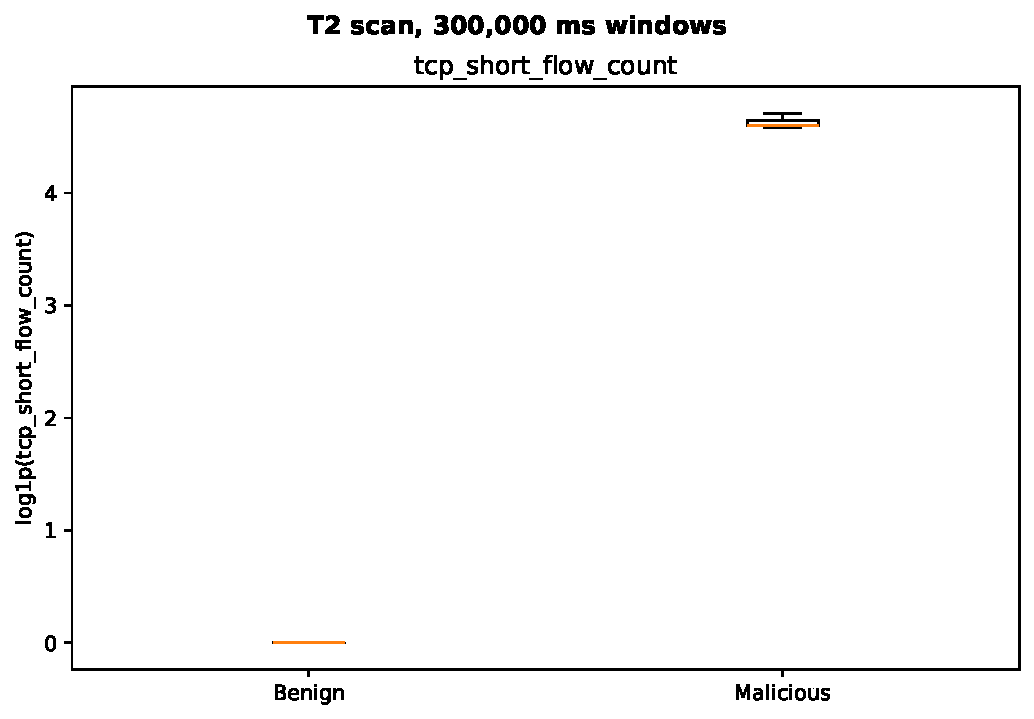
\includegraphics[width=\linewidth]{figures/boxplots_t2_scan_300000ms.pdf}
        \small (a) 
    \end{minipage}
    \hfill
    \begin{minipage}{0.49\textwidth}
        \centering
        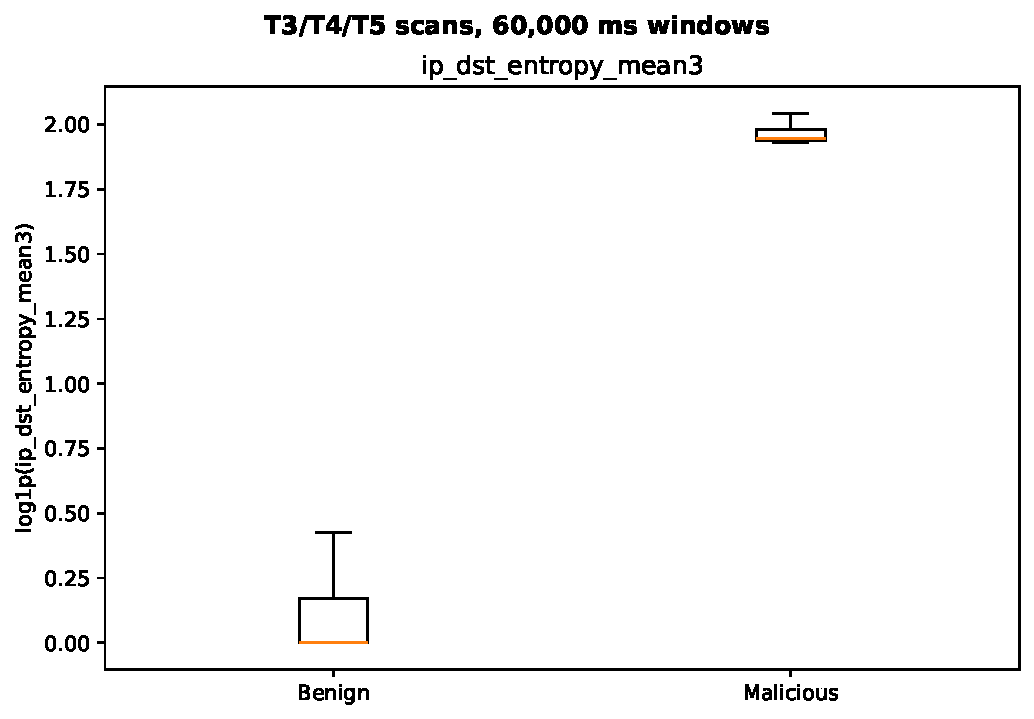
\includegraphics[width=\linewidth]{figures/boxplots_t3_t4_t5_scans_60000ms.pdf}
        \small (b) 
    \end{minipage}


        \end{minipage}
    \end{adjustbox}
    \captionsetup{width=1.3\textwidth}
    \caption{Benign--malicious boxplot comparisons for selected reconnaissance-related features. 
(a) \texttt{tcp\_short\_flow\_count} for the T2 attack using 5-minute windows. 
(b) \texttt{ip\_dst\_entropy\_mean3} for the T3/T4/T5 attacks using 1-minute windows. 
}
    \label{fig:selected_feature_boxplots}
\end{figure}

The ranked summaries of each attack group and window, were used to identify feature families that consistently distinguished reconnaissance from benign traffic. Some of the strongest recurring features were \feat{ip\_dst\_entropy} and \feat{ip\_dst\_entropy\_mean3} representing destination spread, \feat{tcp\_short\_flow\_rate} and \feat{tcp\_short\_flow\_rate\_mean3} representing short-lived TCP scan behavior, and \feat{no\_reply\_packet\_score} and \feat{outbound\_ratio} representing failed or asymmetric communication. Two of these features are illustrated as boxplots in Figure~\ref{fig:selected_feature_boxplots}, visualizing the separation. Based on this information, candidate feature sets were constructed to cover multiple aspects of reconnaissance behavior while limiting redundancy between strongly related features.

This resulted in three types of feature sets. First, general-purpose sets, combining the strongest non-redundant features. Second, attack specific sets emphasizing particular behavior, such as fast and broad scans, stealthy and slow scans, or horizontal host discovery. The last type, isolated specific signal families, such as entropy-only (ADAM), or asymmetry-only groups to get more information on which underlying reconnaissance behaviors contributed most to detection. It is important to clarify that the test split was not used during this feature-set construction process in order to avoid leakage. The exact feature sets can be observed in~\ref{app:feature_sets}.


\section{Anomaly Detection Models}
All models in this section are evaluated in a one-class anomaly detection setting. During training, the models do not rely on labeled data as they are only trained on benign windows, learning a reference of what normal traffic in a specific environment looks like and assigning an anomaly score to unseen windows based on their deviation from this benign reference. Ground-truth labels are introduced only after scoring, in order to evaluate performance.

\subsection{k-Nearest Neighbors}
As discussed in Section [LITERATURE REVIEW], k-Nearest Neighbors (k-NN) is traditionally a supervised learning algorithm, where a new sample is classified based on the labels of its closest neighbors in the training data. However, the same distance-based principle can also be used for one-class anomaly detection.  In that case,the training phase does not involve learning model weights. Instead, the model stores the benign training observations in the selected feature space. During evaluation, each new sample is compared to these stored benign observations using a distance metric. If the sample is close to previously observed normal behavior, it receives a low anomaly score. If it is far from the benign reference set, it receives a high anomaly score. A threshold is then used to decide when this distance is large enough for the window to be considered anomalous.

This principle is reflected in our implementation. The k-NN model is fitted only on the benign training split for which training data is first sorted chronologically by \texttt{window\_start\_ts} and \texttt{window\_id}. The first 80\% of the sorted benign training data is used to build the nearest-neighbor reference set, while the remaining 20\% is kept aside for threshold calibration. This calibration subset is still benign, but is not used to fit the k-NN model itself. After fitting, the model is applied to the calibration subset to estimate the range of distance scores that can still occur under normal behavior. Different percentile thresholds are then tested based on this benign score distribution.

Features are scaled using \texttt{RobustScaler}~\cite{pedregosa_scikit-learn_nodate}, which is fitted only on the 80\% reference subset and then applied unchanged to the calibration and evaluation data. This scaler centers each feature around its median and scales it according to the interquartile range, meaning the spread between the 25th and 75th percentiles. Robust scaling was chosen because derived features may contain extreme values even in benign traffic, the effect of which is contained with this method. The nearest-neighbor search is implemented using the \texttt{NearestNeighbors} class from \texttt{scikit-learn}~\cite{pedregosa_scikit-learn_nodate}, configured with Euclidean distance. Meira et al. empirically validated the use of standard Euclidean distance as the core distance metric when successfully applying One-Class Nearest Neighbor algorithms to network intrusion detection datasets~\cite{meira_performance_2020}. For each input sample, the distances to the \(k\) nearest benign reference samples is computed, by averaging the score to this \(k\) nearest neighbors.
\subsubsection{ADAM}
\label{sec:ADAM}
An additional k-NN variant was included for evaluation based on the feature representation proposed in ADAM. ADAM combines entropy-based traffic profiling with unsupervised anomaly detection for DDoS mitigation in software-defined cyber-physical systems. Normal traffic is represented using entropy based features over the network and transport layer, and it selects k-NN as the anomaly detection modules because of its balance between time overhead and detection affectiveness~\cite{cai_adam_2023}. In order to evaluate the effectiveness of the ADAM proposed feature set, some experiments were run exclusevily using features form the Entropy group in Table~\ref{tab:feature_groups}.



\subsection{Outlier-aware Denoising Autoencoder}
The next anomaly detection approach is based on the the CPS-GUARD method, which uses a semi-supervised deep autoencoder together with an outlier aware threshold selection procedure~\cite{catillo_cps-guard_2023}. Autoencoders are neural networks trained to reconstruct their own input. In anomaly detection, the underlying assumption is that the model trained on benign data will learn to reconstruct normal behavior well, while windows that differ from this learned normal behavior will result in a larger reconstruction error. This error can therefore be used as an anomaly score.

The model is again trained only on benign training windows. The selected input features are first scaled using a preprocessing pipeline consisting of \texttt{RobustScaler} followed by \texttt{MinMaxScaler} with a target range of \([-1,1]\). Robust scaling is used to reduce the influence of extreme feature values, while the min-max scaling step matches the range of the autoencoder output layer, which uses a \texttt{tanh} activation function.

The autoencoder follows a symmetric encoder-decoder structure. Several architectures are evaluated, including the original CPS-GUARD-style \(N\)-36-6-36-\(N\) architecture but also larger or smaller variants, where \(N\) is the number of selected input features. In this notation, \(N\) denotes the number of selected input features. The architecture therefore maps an \(N\)-dimensional input vector to a first hidden layer with 36 neurons, compresses it to a 6-neuron bottleneck representation, expands it again to 36 neurons, and finally reconstructs an \(N\)-dimensional output vector. The hidden layers use ReLU activations, while the output layer uses \texttt{tanh}.The model is trained with mean squared error as reconstruction loss and RMSProp as optimizer. To reduce overfitting to the benign training windows, dropout is applied after the first two hidden layers, as well as Gaussian input noise as a regularization mechanism. A diagram of this model initialized with \(N\)-36-6-36-\(N\) architecture is depicted in Figure~\ref{fig:cpsguard_autoencoder_architecture}

\begin{figure}[htbp]
\centering
\begin{adjustbox}{width=\textwidth}
\begin{tikzpicture}[
    node distance=1.15cm,
    every node/.style={font=\small},
    layer/.style={
        draw,
        rounded corners,
        align=center,
        minimum width=2.0cm,
        minimum height=0.9cm
    },
    reg/.style={
        draw,
        dashed,
        rounded corners,
        align=center,
        minimum width=1.8cm,
        minimum height=0.75cm,
        font=\footnotesize
    },
    arrow/.style={-{Latex[length=2mm]}, thick}
]

\node[layer] (input) {Input\\$N$ features};
\node[reg, right=of input] (noise) {Gaussian\\noise};
\node[layer, right=of noise] (enc1) {Dense 36\\ReLU};
\node[reg, right=of enc1] (drop1) {Dropout};
\node[layer, right=of drop1] (bottleneck) {Dense 6\\ReLU\\Bottleneck};
\node[reg, right=of bottleneck] (drop2) {Dropout};
\node[layer, right=of drop2] (dec1) {Dense 36\\ReLU};
\node[layer, right=of dec1] (output) {Output\\$N$ features\\tanh};

\draw[arrow] (input) -- (noise);
\draw[arrow] (noise) -- (enc1);
\draw[arrow] (enc1) -- (drop1);
\draw[arrow] (drop1) -- (bottleneck);
\draw[arrow] (bottleneck) -- (drop2);
\draw[arrow] (drop2) -- (dec1);
\draw[arrow] (dec1) -- (output);

\node[above=0.25cm of enc1] {\textbf{Encoder}};
\node[above=0.25cm of dec1] {\textbf{Decoder}};

\end{tikzpicture}
\end{adjustbox}
\caption{CPS-GUARD-style autoencoder architecture used for reconstruction-based anomaly detection. The \(N\)-dimensional feature vector is regularized using Gaussian noise, compressed into a lower-dimensional bottleneck representation, and then reconstructed at the output. Dropout is applied after the first two hidden layers during training.}
\label{fig:cpsguard_autoencoder_architecture}
\end{figure}

For threshold selection, the benign training data is divided into an autoencoder training subset and a separate benign threshold-calibration subset, which is excluded from training. After training, the calibration subset is passed through the autoencoder and each calibration window receives a reconstruction error, which represents a range of scores that can still occur at benign inputs. Then Isolation Forest is applied to the calibration subset to separate benign calibration samples from outliers~\cite{catillo_cps-guard_2023}. The reconstruction errors of these two groups are used by the threshold selection procedure to choose a final anomaly threshold. This way, instead of directly selecting a fixed percentile of all benign reconstruction errors, possible outliers in the benign calibration set are filtered out. Different contamination values were tested for this step.



\subsection{K-means}
The final model used is based on K-means clustering. K-means is an unsupervised clustering algorithm that partitions the training data into \(k\) clusters by assigning samples to the nearest cluster centroid. Although K-means is primarily a clustering algorithm, it can be adapted to one-class anomaly detection by treating the distance to the nearest benign cluster centroid as an anomaly score~\cite{meira_performance_2020}. Then, during evaluation, a new sample is compared to these centroids. Samples close to one of the benign clusters receive a low anomaly score, while samples far away from all learned centroids receive a high anomaly score.

As repeated for the previous models, the K-means model is fitted only on the benign training split. The training data is first sorted chronologically by \feat{window\_start\_ts} and, \feat{window\_id} of which the first 80\%  is used to fit the K-means model, while the remaining 20\% is kept aside as a benign calibration subset for threshold selection. Features are scaled using \feat{RobustScaler}, which is fitted only on the 80\% model-fitting subset and then applied unchanged to the calibration and evaluation data.

After training, each calibration sample is assigned an anomaly score equal to its Euclidean distance to the nearest cluster centroid. The anomaly threshold is then selected as a tested quantile of these benign calibration distances. During evaluation, each validation or test window is scaled using the same scaler and assigned its nearest-centroid distance. A window is classified as anomalous when this distance exceeds the selected threshold.

Several values for the number of clusters are tested. Smaller values force the model to represent benign behavior using only a few broad traffic profiles, while larger values allow the model to capture more fine-grained modes of normal behavior. Similarly to the k-NN approach, different threshold quantiles are evaluated to study the trade-off between detecting malicious windows and limiting false positives on benign traffic.  The implementation uses the \texttt{MiniBatchKMeans} class from \texttt{scikit-learn}~\cite{pedregosa_scikit-learn_nodate}.




% talk about the zscore and why we don't use it.




\section{Experimental Configuration}
With the defined models, there are still several design choices that can influence their detection performance. These include the feature set, aggregation window length, anomaly threshold, and model-specific parameters such as the number of nearest neighbors, number of K-means clusters, autoencoder architecture, and Isolation Forest contamination value. In order  to meaningfully select the model that would best perform for reconnaissance detection on conntrack-derived OT traffic, all possible combination of these parameters were explored. 

The sweeps are organized around four main dimensions. First, multiple aggregation window sizes are evaluated in order to study how temporal granularity affects detection. Shorter windows may capture short scanning bursts more precisely, while longer windows may smooth traffic behavior and make low-rate reconnaissance activity more visible. Second, several feature sets are tested, ranging from more general reconnaissance based sets, to more case specialized sets as discussed in~\ref{sec:features}. Third, each model is evaluated under multiple threshold settings. For distance-based models (such as K-NN or K-means), thresholds are selected as quantiles of the benign calibration score distribution, and for the autoencoder different Isolation Forest contamination values are tested. Finally, model-specific parameters are varied, such as \(k\) for k-NN, the number of clusters for K-means, and the hidden-layer dimensions of the autoencoder.

After exploring all these possibilities, the validation data is used to evalute which configurations show the most promising results. Based on this parameters are modified as suited and certain feature sets are added or removed for the next sweeps. The validation data is also used to select the best model/parameter combinations to be advanced to the testing phase.

\section{Evaluation Metrics}



The models are evaluated using both window-level and range-lavel metrics. Window-level F1 treats each window independently which can be limiting for reconnaissance detection, because an attack is usually not a single isolated window, but an activity that unfolds over a continuous time interval. A detector that raises at least one alarm during such an interval may already be useful from an operational perspective, even if it does not flag every malicious window. Similarly, a model may obtain a good window level F1-score while producing several separate false alarm intervals, which would be less desirable for an operator. This issue is also discussed by Fung et al.~\cite{atluri_perspectives_2022} , who show that point-wise F1 can give a misleading impression of anomaly detection performance in ICS time-series settings, and argue that range-based metrics better capture operational objectives such as reducing false alarms and detecting attack intervals.

Window-level precision, recall and F1-score are computed from the number of true positives, false positives and false negatives over all evaluated windows. A true positive (TP) is a window that overlaps with an attack interval and is predicted as anomalous. A false positive (FP) is a benign window that is incorrectly predicted as anomalous, while a false negative (FN) is an attack window that is not detected. These metrics provide a more fine grained view and are useful for comparing how precisely each model identifies anomalous windows. 

For the discussed range based precision, recall and F1-score, the true labels and model predictions are first processed separately for each source host. Consecutive positive windows are grouped into temporal ranges after sorting by timestamp. A true attack range is counted as detected when at least one predicted anomalous range overlaps with it. Predicted anomalous ranges that do not overlap with any true attack range are counted as range-level false positives, while true attack ranges without any overlapping prediction are counted as range-level false negatives. Hence, the range-based metric used here therefore follows an event-detection interpretation. It does not require every malicious window inside an attack interval to be classified correctly.


Window-level precision, recall and F1-score are defined as:

\begin{equation}
    \text{Precision} = \frac{TP}{TP + FP}
\end{equation}

\begin{equation}
    \text{Recall} = \frac{TP}{TP + FN}
\end{equation}

\begin{equation}
    F_1 = 2 \cdot \frac{\text{Precision} \cdot \text{Recall}}
    {\text{Precision} + \text{Recall}}
\end{equation}

where \(TP\), \(FP\), and \(FN\) are counted over individual source-host windows.


The same precision, recall and F1-score definitions are then applied at the range level:



\begin{equation}
    \text{Range Precision} = 
    \frac{TP_{\text{range}}}{TP_{\text{range}} + FP_{\text{range}}}
\end{equation}

\begin{equation}
    \text{Range Recall} = 
    \frac{TP_{\text{range}}}{TP_{\text{range}} + FN_{\text{range}}}
\end{equation}

\begin{equation}
    F_{1,\text{range}} =
    2 \cdot
    \frac{\text{Range Precision} \cdot \text{Range Recall}}
    {\text{Range Precision} + \text{Range Recall}}
\end{equation}

A predicted range \(P=[p_s,p_e]\) overlaps a true attack range \(T=[t_s,t_e]\) when:
\[
p_s \leq t_e \land p_e \geq t_s .
\]

Both metrics are reported because they provide complementary views of the same predictions. Window-level F1 evaluates each source-host window separately, while range-level F1 summarizes consecutive detections into temporal alarm ranges. Differences between them are therefore interpreted as different perspectives on model performance, rather than as contradictory results.





% 3.6 Anomaly Detection Models
%     3.6.1 KNN-Based Detector
%     3.6.2 Isolation Forest
%     3.6.3 Deep Autoencoder + Isolation Forest
%     3.6.4 ADAM-Inspired Statistical Baseline
%     3.6.5 Optional: K-Means Baseline

% 3.7 Threshold Selection and Hyperparameter Tuning

% 3.8 Evaluation Metrics
% SINCE we are aggragatng features we are already doing a knd of range based metric but here then the range based is for the entre range of the attack.
%     3.8.1 Point-Based Metrics
%     3.8.2 Range-Based Metrics
%     3.8.3 Comparison Between Metric Types

% 3.9 IT Comparison Dataset

% 3.10 Implementation Details and Reproducibility
%   -dask